% ! Tex program = xelatex
\documentclass{article}
% 中文
% \usepackage[UTF8]{ctex}

% For more choices
% --------------definations-------------- %
\def\*#1{\boldsymbol{#1}}
\def\+#1{\mathcal{#1}} 
\def\-#1{\mathrm{#1}}
\def\=#1{\mathbb{#1}}
% Domains
\def\RR{\mathbb{R}}
\def\EE{\mathbb{E}}
\def\Ex{\mathbb{E}}
\def\CC{\mathbb{C}}
\def\NN{\mathbb{N}}
\def\ZZ{\mathbb{Z}}
% Newcommand
\newcommand{\inner}[2]{\langle #1,#2\rangle} 
\newcommand{\numP}{\#\mathbf{P}} 
\renewcommand{\P}{\mathbf{P}}
\newcommand{\Var}[2][]{\mathbf{Var}_{#1}\left[#2\right]}
\newcommand{\E}[2][]{\mathbf{E}_{#1}\left[#2\right]}
\renewcommand{\emptyset}{\varnothing}
\newcommand{\ol}{\overline}
\newcommand{\argmin}{\mathop{\arg\min}}
\newcommand{\argmax}{\mathop{\arg\max}}
\newcommand{\abs}[1]{\qty|#1|}
\newcommand{\defeq}{\triangleq} % triangle over =
\def\deq{\xlongequal{def}} % 'def' over =
\def\LHS{\text{LHS}}
\def\RHS{\text{RHS}}
\def\angbr#1{\left\langle#1\right\rangle} % <x>
\def\set#1{\qty{#1}}

\usepackage{fancyhdr}
\pagestyle{fancy}
% \fancypagestyle{mainFancy}{
%     \fancyhf{}
%     \renewcommand\headrulewidth{.5pt}       % 页眉横线
%     \renewcommand\footrulewidth{0pt}
%     \fancyhead[OC]{\fzkai{\leftmark}}       % 页眉章标题
%     \fancyhead[EC]{\fzkai{\@title}}         % 页眉文章题目
% 	\lhead{\fzkai{author}}
%     \fancyhead[OR,EL]{\thepage}                 % 页眉编号
%     \fancyfoot[r]{\thumb} % 将拇指放到没有被使用的页眉或页脚处
% }
\fancyhead[L]{\slshape{Haoyu Zhen}}

% theorems
\usepackage{thmtools}
\usepackage{thm-restate}
\usepackage[framemethod=TikZ]{mdframed}
\mdfsetup{skipabove=1em,skipbelow=0em, innertopmargin=12pt, innerbottommargin=8pt}

\theoremstyle{definition}

\declaretheoremstyle[headfont=\bfseries\sffamily, bodyfont=\normalfont,
	mdframed={
		nobreak,
		backgroundcolor=brown!14,
		topline=false,
		rightline=false,
		leftline=true,
		bottomline=false,
		linewidth=2pt,
		linecolor=brown!180,
	}
]{thmbrownbox}

\declaretheoremstyle[headfont=\bfseries\sffamily, bodyfont=\normalfont,
	mdframed={
		nobreak,
		backgroundcolor=Blue!4,
		topline=false,
		rightline=false,
		leftline=true,
		bottomline=false,
		linewidth=2pt,
		linecolor=NavyBlue!120,
	}
]{thmbluebox}

\declaretheoremstyle[headfont=\bfseries\sffamily, bodyfont=\normalfont,
	mdframed={
		nobreak,
		backgroundcolor=Green!5,
		topline=false,
		rightline=false,
		leftline=true,
		bottomline=false,
		linewidth=2pt,
		linecolor=OliveGreen!120,
	}
]{thmgreenbox}

\declaretheoremstyle[headfont=\bfseries\sffamily, bodyfont=\normalfont,
	mdframed={
		nobreak,
		topline=false,
		rightline=false,
		leftline=true,
		bottomline=false,
		linewidth=2pt,
		linecolor=OliveGreen!120,
	}
]{thmgreenline}

\declaretheoremstyle[headfont=\bfseries\sffamily, bodyfont=\normalfont,
	mdframed={
		nobreak,
		topline=false,
		rightline=false,
		leftline=true,
		bottomline=false,
		linewidth=2pt,
		linecolor=NavyBlue!70,
	}
]{thmblueline}

\declaretheorem[numberwithin=section, style=thmbrownbox, name={\color{Brown}Definition}]{defi}
\declaretheorem[numberwithin=section, style=thmgreenbox, name={\color{OliveGreen}Law}]{law}
\declaretheorem[numberwithin=section, style=thmbluebox, name={\color{Blue}Corollary}]{cor}
\declaretheorem[numberwithin=section, style=thmgreenline, name={\color{OliveGreen}Property}]{prt}
\declaretheorem[numberwithin=section, style=thmbluebox, name={\color{Blue}Proposition}]{prp}
\declaretheorem[numberwithin=section, style=thmbluebox, name={\color{Blue}Theorem}]{thm}
\declaretheorem[numberwithin=section, style=thmbluebox, name={\color{Blue}Lemma}]{lemma}
\declaretheorem[numberwithin=section, style=thmbrownbox,  name={\color{Brown}Example}]{eg}
\declaretheorem[numberwithin=section, style=thmgreenline, name={\color{OliveGreen}Remark}]{remark}
\declaretheorem[numbered=no,style=thmblueline, name={\color{NavyBlue!70}Proof},qed=$\square$]{prf}
\numberwithin{equation}{section}


\usepackage{titlesec}
\graphicspath{{img/}}

\setstretch{1.2}
\begin{document}
\title{\vspace{5cm}Computer Graphics Lecture Notes}
\maketitle

\clearpage
\tableofcontents
\section*{Acknowledgement}
These Notes contain material developed and copyright by CS148: Introduction to Computer Graphics and Imaging, Stanford University. To get more information, you could visit the course website: \url{https://web.stanford.edu/class/cs148/index.html}.

\section{Geometry}
\textbf{Loop Subdivision}
\begin{itemize}
	\vspace{-0.5em}\item Subdivide each triangle into 4 sub-triangles
	\vspace{-0.5em}\item Move both the old/new vertices
	\vspace{-0.5em}\item Repeat (if desired)
	\vspace{-0.5em}\item C2 continuity almost everywhere (except at some extraordinary vertices where itʼs only C1)
\end{itemize}

\vspace{0.5em}\textbf{Cardinal Cubic Splines}

4 control points $\{p_{i-1},p_{i},p_{i+1},p_{i+2}\}$. What we want is  $f(u)=a_0+a_1u+a_2u^2+a_3u^3$ such that
\[
	f(0)=p_i\qcomma f(1)=p_{i+1} \qcomma f'(0)=s(p_{i+1}-p_{i-1}) \qand f'(1)=s(p_{i+2}-p_i)
.\]

\subsection{Transformation}
\textbf{Rotation}
\[
	R_x=\mqty(1 & 0 & 0 \\ 0 & \cos\theta & -\sin\theta \\ 0 & \sin\theta & \cos\theta)
	\qcomma 
	R_y=\mqty(\cos\theta & 0 & \sin\theta \\ 0 & 1 & 0 \\ -\sin\theta & 0 & \cos\theta)
	\qand
	R_z=\mqty(\cos\theta & -\sin\theta & 0 \\ \sin\theta & \cos\theta & 0 \\ 0 & 0 & 1)
\] 
\textbf{Scaling}
\[
	S=\mqty(s_1 & 0 & 0 \\ 0 & s_1 & 0 \\ 0 & 0 & s_3)
.\] 
\textbf{Homogeneous Coordinates}
 \[
	 \vec{p}_H=\mqty(x & y & z & 1)^T
.\] 
Then we have
\[
	\mqty(\*M & \*{t} \\ \*O & 1)\mqty(\*x \\ 1) = \mqty(\*M\*x+\*t \\ 1)
\] where $\*M\in\RR^{3\times 3}$ and  $\*O\in\RR^{1\times3}$.

\section{Color and Image}
\subsection{Rasterization}
For each pixel, if the center of the pixel is inside the triangle, consider it part of the triangle (and color it with the triangleʼs color.)
\subsection{Phong Reflection Model}
\[
	\begin{aligned}
		C&=
		\text{ambient}+\text{diffuse}+\text{specular}
		\\&=
		k_a+k_d\max(0,\hat{N}\cdot\hat{L})+k_s\qty(\max(0,\hat{V}\cdot\hat{R}))^\alpha
	\end{aligned}
\]
where $\hat{N}, \hat{L}, \hat{V}$ and $\hat{R}$ are defined as follows.
\begin{figure}[htpb]
	\centering
	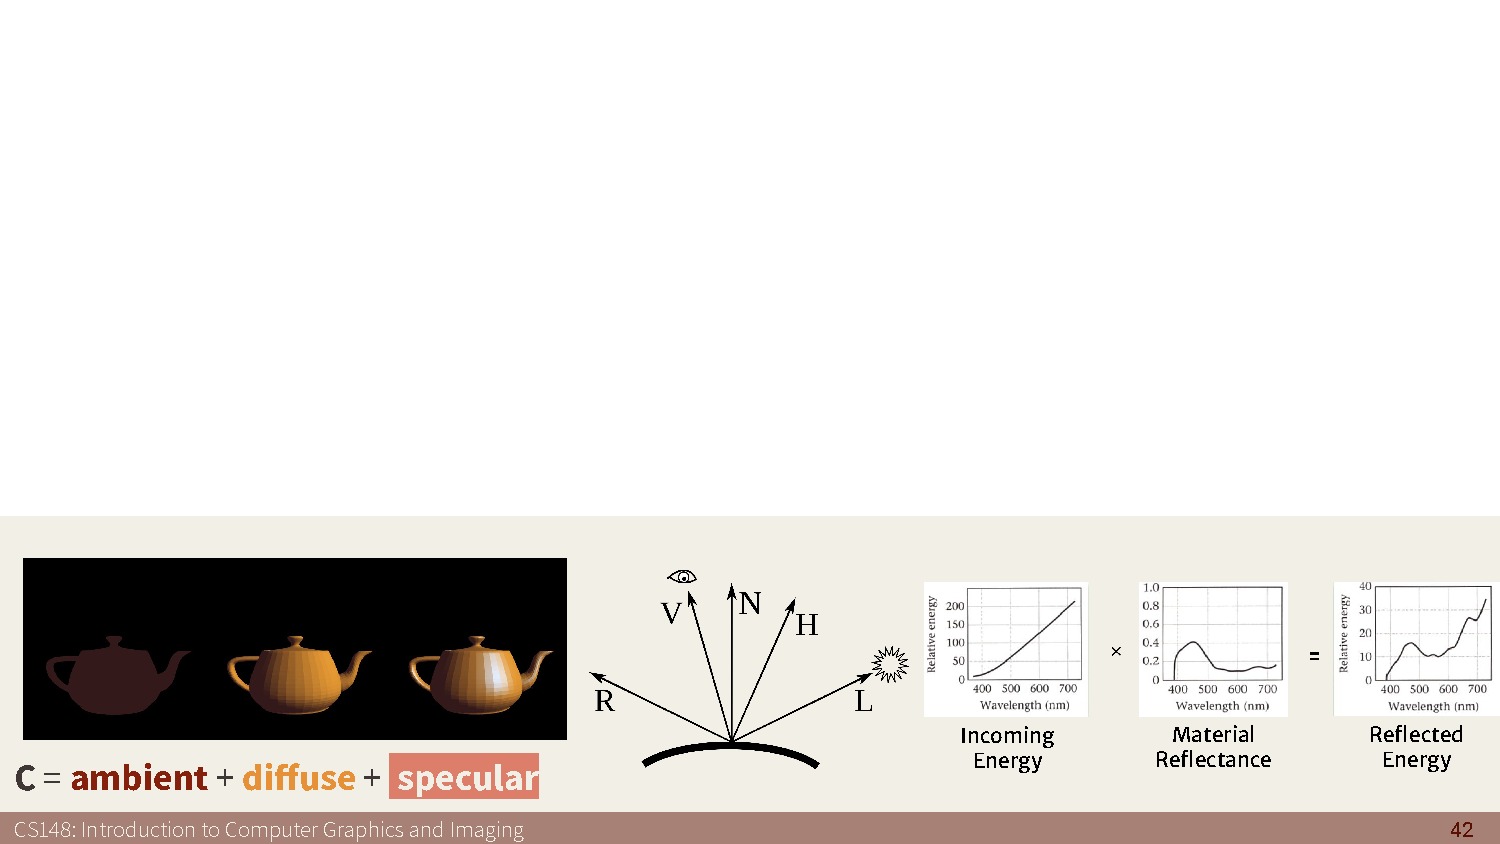
\includegraphics[width=\linewidth]{img/prm.pdf}
	\label{fig:prm}
\end{figure}
\begin{itemize}
	\vspace{-2.5em}\item \textbf{Ambient}: ``Base color''. Light bounces arounf the environment.
	\vspace{-0.5em}\item \textbf{Diffuse}: ``Rough marterial''. Given the same light source, objects look brighter when hit ``perpendicularly''.
	\vspace{-0.5em}\item \textbf{Specular}: ``Shiny material''. Bright highlights when light reflects into our eyes.
\end{itemize}

\section{Camera}
The mathematical form of the projection:
\[
	p_{\-{img}}
	=
	M_{\-{obj}2\-{img}}\cdot p_{\-{obj}}
	=
	M_{\-{cam}2\-{img}}M_{\-{world}2\-{cam}}M_{\-{obj}2\-{world}}\cdot p_{\-{obj}}
\]
\subsection{Camera to Film}
\subsubsection{Modeling the Pinhole Camera}
\[
	P(x,y,z)=\mqty(\flatfrac{hx}{z} & \flatfrac{hy}{z} & h)
.\]
Condsider homogeneous coordinates:
\[
	\mqty(
	1 & 0 & 0 & 0 \\
	0 & 1 & 0 & 0 \\
	0 & 0 & 1 & 0 \\
	0 & 0 & \*{1} & \*{0} \\
	)
	\mqty(x\\y\\z\\1)
	\qor
	\mqty(
	h & 0 & 0 & a \\
	0 & h & 0 & b \\
	0 & 0 & 1 & 0 \\
	0 & 0 & \*{1} & \*{0} \\
	)
	\mqty(x\\y\\z\\1)
.\]
\subsubsection{Viewing Frustrum}
\begin{itemize}
	\item Idea: transform viewing frustrum to an orthographic bounding box
	\item Instead of projecting everything to the plane at fixed depth, project to a cube first
	\item Clip anything thatʼs not within $-1\to 1$
\end{itemize}
\[
	\mqty(x'\\y'\\z'\\w')=
    \mqty(\displaystyle
	\flatfrac{1}{r_x} & 0 & 0 & 0 \\
	0 & \flatfrac{1}{r_y} & 0 & 0 \\
	0 & 0 & \cfrac{d_0+d_1}{d_0-d_1} & \cfrac{2d_0d_1}{d_0-d_1} \\[6pt]
	0 & 0 & \*{-1} & \*{0} \\
	)
	\mqty(x\\y\\z\\1)
.\] 
where we have $r_x$, $r_y$ corresponding to film boundaries, $d_0 / d_1$ being the clipping planes.
\subsubsection{$\*z$-buffer Algorithm}
Then we introduce the \textbf{$\*z$-buffer algorithm}:
\begin{algorithm}[htbp]
	\caption{$z$-buffer algorithm (output: $\+C$ and $\+Z$)}
	\begin{algorithmic}[1]
		\renewcommand{\algorithmicrequire}{\textbf{Input:}}
		\renewcommand{\algorithmicensure}{\textbf{Output:}}
		\renewcommand{\algorithmiccomment}[1]{\hfill\textit{\textcolor{blue}{\##1}}}
		\STATE For all $x$ and $y$, $\+Z(x,t)\gets-\infty$
		\FOR{Each $(x,y,z)$ in each fragment with corresponding color $c$}
		\IF{$\+Z(x,y)<z$}
		\STATE $\+C(x,y)\gets c$ and $\+Z(x,y)\gets z$
		\ENDIF
		\ENDFOR
	\end{algorithmic}
\end{algorithm}

\subsection{The rasterization pipeline}
\begin{enumerate}
	\item Vertex shader outputs vertex attributes and orthogonal clipping space positions
	\item Vertex data assembled into triangles, data outside the viewing frustrum is discarded
	\item For each triangle, rasterize vertex attributes (\textbf{barycentric interpolation})
	\item Fragment shader takes interpolated attributes and computes color
	\item Use the $z$-buffer to help assemble pixel colors into the full image
\end{enumerate}
\begin{figure}[H]
	\centering
	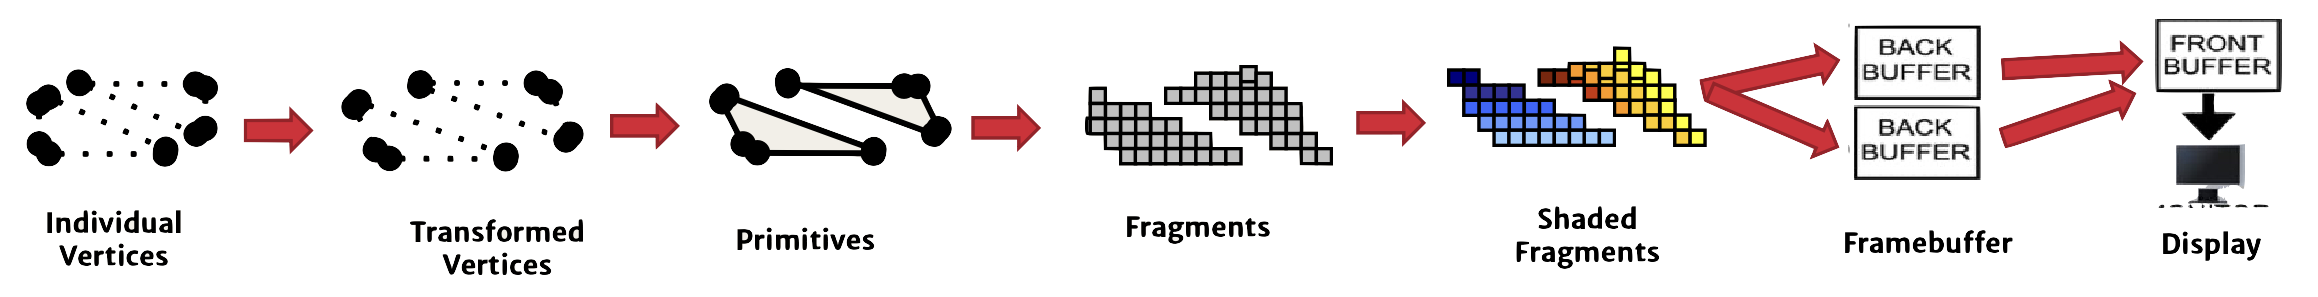
\includegraphics[width=\linewidth]{rasterization.png}
	\label{fig:rasterization}
\end{figure}

\section{Optics}
\begin{defi}
	\textbf{Radiant Intensity} of a light source: $I(\omega)=\dv*{\Phi}{\omega}$
	\begin{itemize}
		\vspace{-0.5em}\item Total light power (exiting a light) per unit solid angle
		\vspace{-0.5em}\item Measure of how strong a (point) light source is
	\end{itemize}
\end{defi}
\begin{defi}
	\textbf{Irradiance} on a surface: $E=\dv*{\Phi}{A}$
	\begin{itemize}
		\vspace{-0.5em}\item Total light power (hitting a surface) per unit surface area.
		\vspace{-0.5em}\item Measure of how much light is hitting a surface.
		\vspace{-0.5em}\item Varies based on distance from the light and the tilting angle of the surface.
	\end{itemize}
\end{defi}
Some engineering approximations are as follows.
\begin{itemize}
	\item BRDF (Bidirectional Reflectance Distribution Function): models how much light is reflected.
	\item BTDF (Bidirectional Transmittance Distribution Function): models how much light is transmitted.
	\item BSSRDF (Bidirectional Surface Scattering Reflectance Distribution Function): combined reflection/transmission model.
\end{itemize}

Now we define the \textbf{lighting equation}:
\[
	L_o(\omega_0)=\sum_{i\in\mathrm{in}}L_{o\text{ due to }i}(\omega_i,\omega_o)
\]
where the BRDF gives each of $L_{o\text{ due to }i}(\omega_i,\omega_o)$.
Then we have
\[
	L_o(\omega_0)=\int_{i\in\mathrm{in}}\mathrm{BRDF}(\omega_i,\omega_0)\dd{E_i(\omega_i)}
	=
	\int_{i\in\mathrm{in}}\mathrm{BRDF}(\omega_i,\omega_0)L_i\cos\theta_i\dd{\omega_i}
.\] 

Diffuse Materials: a surface reflects light equally in all directions. I.e., $\mathrm{BRDF}=\mathrm{Const}$.

\section{Ray Tracing}
\subsection{Constructing Rays}
Shoot a ray for each pixel:
\[
    R(t)=A+(P-A)t
\] where $A$ is the aperture, P is the pixel center and $t$ is defined  $t\in[0,+\infty)$.

\subsection{Acceleration}
\textbf{Parallelization}: each ray is independent of any other ray


	
\end{document}
